\section{Encoding FMUs by timed automata}
\label{sec:fmi}
We give the syntax and semantics of FMU and timed automata. In order to verify the  execution of FMUs. We propose to encode FMUs by timed automata. In section \ref{sec:sysml}, we verify the network of timed automata in UPPAAL.
\subsection{FMU}
FMU is the model component which implements the methods defined in the FMI API \cite{Tripakis15}. Here, we present the syntax and semantics of FMU. The aim is to encode FMU into timed automata based on their semantics. 
\begin{definition}
\textbf{FMU syntax}
We recall the definition of FMU. An FMU is a tuple $F=(L,U,Y,D,l_{0},set,get,doStep)$, where:
\end{definition}
\begin{itemize}
\item
$L$ denotes the set of locations of $F$. 
\item
$U$ denotes the set of input port variables of $F$. Note that an element $u \in U$ is a variable, not a value, which ranges over a set of values $\mathbb{V}$. 
\item
$Y$ denotes the set of output port variables of $F$. Each $y \in Y$ ranges over the same set of values $\mathbb{V}$.
\item
$D \subseteq U \times Y$ denotes a set of input-output dependencies. $(u,y) \in D $ means that the output y is directly dependent on the value of u. The $I/O$ dependency information is used to ensure that a network of FMUs does not contain cyclic dependencies, and also to identify the order in which all variables are computed during a step.
\item
$l_{0} \in L$ denotes the initial location of $F$.
\item
$set : L \times U \times \mathbb{V} \rightarrow L$ denotes the function that sets the value of an input variable. Given current location $l \in L$, input variable $u \in U$, and value $v \in \mathbb{V}$, it returns the new location obtained by setting $u$ to $v$.
\item
$get : L \times Y \rightarrow \mathbb{V}$ denotes the function that returns the value of an output variable. Given location $l \in L$ and output variable $y \in Y$, $get(l,y)$ returns the value of $y$ in $l$.
\item
$doStep : L \times \mathbb{R}_{\geqslant{0}} \rightarrow L \times \mathbb{R}_{\geqslant{0}}$ denotes the function that implements one simulation step. Given current location $l$,~and a non-negative real value $h \in \mathbb{R}_{\geqslant{0}}$,~    $doStep(l,h)$ returns a pair $(l^{\prime},h^{\prime})$ such that:
\\
When $h^{\prime} = h$, it indicates that $F$ accepts the time step $h$ and reaches the new location $l^{\prime}$;
\\
When $0 \leqslant h^{\prime} < h$, this means that $F$ rejects the time step $h$, but making partial progress up to $h^{\prime}$, and reach the new location $l^{\prime}$.
\end{itemize}
\begin{definition}
\textbf{FMU semantics}
Given the FMU $F=(L,U,Y,D,l_{0},set,get,doStep)$,
\end{definition} 
The behavior of $F$ depends on the functions $doStep$, which is a function of a timed input sequence (TIS). A TIS is an infinite sequence 
$v_{0}h_{1}v_{1}h_{2}v_{2}h_{3}...$
of alternating input assignments $v_{i}$, and time delays $h_{i}$. An input assignment is the value of function $v : U \rightarrow \mathbb{V}$. That is, $v$ assigns a value to every input variable in $U$.
A TIS denotes a running of $FMU$, which is an infinite sequence of quadruples $(t,l,v,v^{\prime})$, where $t \in \mathbb{R}_{\geqslant{0}}$ is a time instant, $l \in L$ is a location of $F$, $v$ is an input assignment, and $v^{\prime} : Y \rightarrow \mathbb{V}$ is an output assignment
 
TIS := $(t_{0},l_{0},v_{0},v_{0}^{\prime})(t_{1},l_{1},v_{1},v_{1}^{\prime})(t_{2},l_{2},v_{2},v_{2}^{\prime})...$ is
defined as follows:
\begin{itemize}
\item
$t_{0} = 0$ and $l_{0}$ is the initial location of $F$.
\item
For each $i \geqslant 1$, $t_{i} = t_{0} + \sum_{k = 1}^i h_{k}$
\item
Given the current location $l_{i}$, the function $set$ is used to set all input variables to the values specified by $v$. Then $F$ reaches a new location $l_{i}^{\prime}$. The function $get$ is used to get the values of all output variables $v_{i}^{\prime}$.
\item 
We assume that $doStep(l_{i}, h_{i+1}) = (l_{i+1},h_{i+1})$ based on the assumption that every $h_{i}$ is accepted by $F$, $F$ will reach the next location $l_{i+1}$.
\end{itemize}
\subsection{Timed Automata}
Timed automata (TA) \cite{BehrmannDLHPYH06} is a theory to model the behavior of real-time systems. Its definition provides a powerful way to annotate state-transition graphs with many real-valued clocks. In this section, we introduce the syntax and semantics of timed automata. In section \ref{sec:sysml}, we will model the master algorithm and encode the FMUs of our case study with the network of TA, so that we can use the model checker UPPAAL to analyse models.
\begin{definition}
\textbf{Timed automata syntax}
A timed automaton is a tuple $\textit{A}=(S,X,s_{0},E,E_{O},E_{I},I)$, where:
\end{definition}
\begin{itemize}
\item
S is a finite set of states;
\item
X is a finite set of clocks;
\item
$s_{0}\in  S$ is an initial state;
\item
The set of guards $G(x)$ is defined by the grammar $g := x \bowtie c \mid g \land g$, where $x \in X$, $c \in \mathbb{N}$ and $\bowtie~\in \{<,\leqslant,\geqslant,>\}$. $E\subseteq S \times G(X) \times 2^X \times S$ is a set of edges labelled by guards and a set of clocks to be reset;
\item
$E_{O}$ is a set of input events.
\item
$E_{I}$ is a set of output events.
\item
$I : S \rightarrow G(X)$ assigns invariants to clocks.
\end{itemize}
A clock valuation is a function $v : X \rightarrow \mathbb{R}_{\geqslant{0}}$. If $\delta \in \mathbb{R}_{\geqslant{0}}$, then $v + \delta$ denotes the valuation such that for each clock $x \in X$, $(v + \delta)(x) = v(x) + \delta$. If $Y \subseteq X$, then $v[Y := 0]$ denotes the valuation such that for each clock $x \in X~Y$, $v[Y := 0 ](x) = v(x)$ and for each clock $x \in Y$, $v[Y := 0](x) = 0$. The satisfaction relation $v \models g$ for $g \in G(x)$ is defined in the natural way.
\begin{definition}
\textbf{Timed automata semantics} 
The semantics of a timed automaton $\textit{A} = (S,X,s_{0},E, \\E_{O},E_{I},I)$ is defined by a transition system $S_{\textit{A}} = (S,s_{0},\rightarrow)$, \end{definition}
where $S = S \times \mathbb{R}_{\geqslant{0}}^X$ is the set of states, $s_{0} = (s_{0},v_{0})$ is the initial state, $v_{0}(x) = 0$ for all $x \in X$, and $\rightarrow \subseteq S \times S$ is the set of transitions defined by :
\begin{itemize}
\item
$(s,v) \xrightarrow{\in(\delta)} (s,v+\delta)$ if $\forall0 \leqslant \delta^{\prime} \leqslant \delta : (v + \delta^{\prime}) \models I(s)$;
\item
$(s,v) \rightarrow(s^{\prime},v[Y := 0])$ if there exists $(s,g,Y,s^{\prime}) \in E$ such that $v \models g$ and $v[Y := 0 ] \models I(s^{\prime})$.
\end{itemize}
The reachability problem for an automaton $A$ and a location $s$ is to decide whether there is a state $(s,v)$ reachable from $(s_{0},v_{0})$ in the transition system $S_{A}$. As usual, for verification purposes, we define a symbolic semantics for timed automata. For universality, the definition uses arbitrary sets of clock valuations.
\subsection{Encoding FMUs by timed automata}
As we can see, there is a semantic gap between FMU and TA. The former focus on the execution sequence of FMU, which specifies the state change process with time passing. The simulation trace of TA is similar as the execution sequence of FMU. Therefore, we can encode FMU with TA to analyse the behavior of FMU component without 
exploring its internal structure.

Given an FMU $F=(L,U,Y,D,l_{0},set,get,doStep)$, we model this FMU by a timed automaton $A = (S,X,s_{0},E,E_{O},E_{I},I)$, where:
\begin{itemize}
\item
$S$ is a set of finite locations. Note that a state of TA is the abstraction of a location in $F$.
\item
The initial state $s_{0}$ which $t:=0 \vert t \in X$ is such that $l$ is set to $l_{0}$. 
\item
Each input variable $u \in U$ ranges over $E_{I} \cup \{absent\}$.
\item
Each output variable $y \in Y$ ranges over $E_{O} \cup \{absent\}$.
\item
An input event in $e \in E_{O}$ is such that the function $set$ of $F$ sets the input variable $u$ to a given value. 
\item
An output event in $e \in E_{I}$ indicates that the function $get$ of $F$ gets the output variable $y$. The set of values in the $E_{I}$ is the $Y$.  
\item
The communication with input and output events in TA is the same as the I/O dependencies information in FMU. $(u,y) \in D$ denotes that output y depend on input u. The output events also depend on the input events.
\item
For any $e \in E$ of A, there is a transition $s \xrightarrow{e} s^{\prime}$, which may be found after the function $doStep$ is executing. For instance, if there is a transition $l \xrightarrow{e} l^{\prime}$, at the same time $doStep(l,h)$ may be called which indicates that $F$ accepts the time step $h$ and reaches the new location $l^{\prime}$. However, $F$ maybe rejects the time step for the reason which we have discussed above and this process can also be described in the TA. If there is a rollback behavior happens after the $F$ rejects the time step $h$, the transition in TA could be a edge $s \xrightarrow{e} s$, which denotes that a state travels to itself.

\end{itemize}
\begin{figure}[htbp]
	\centering	{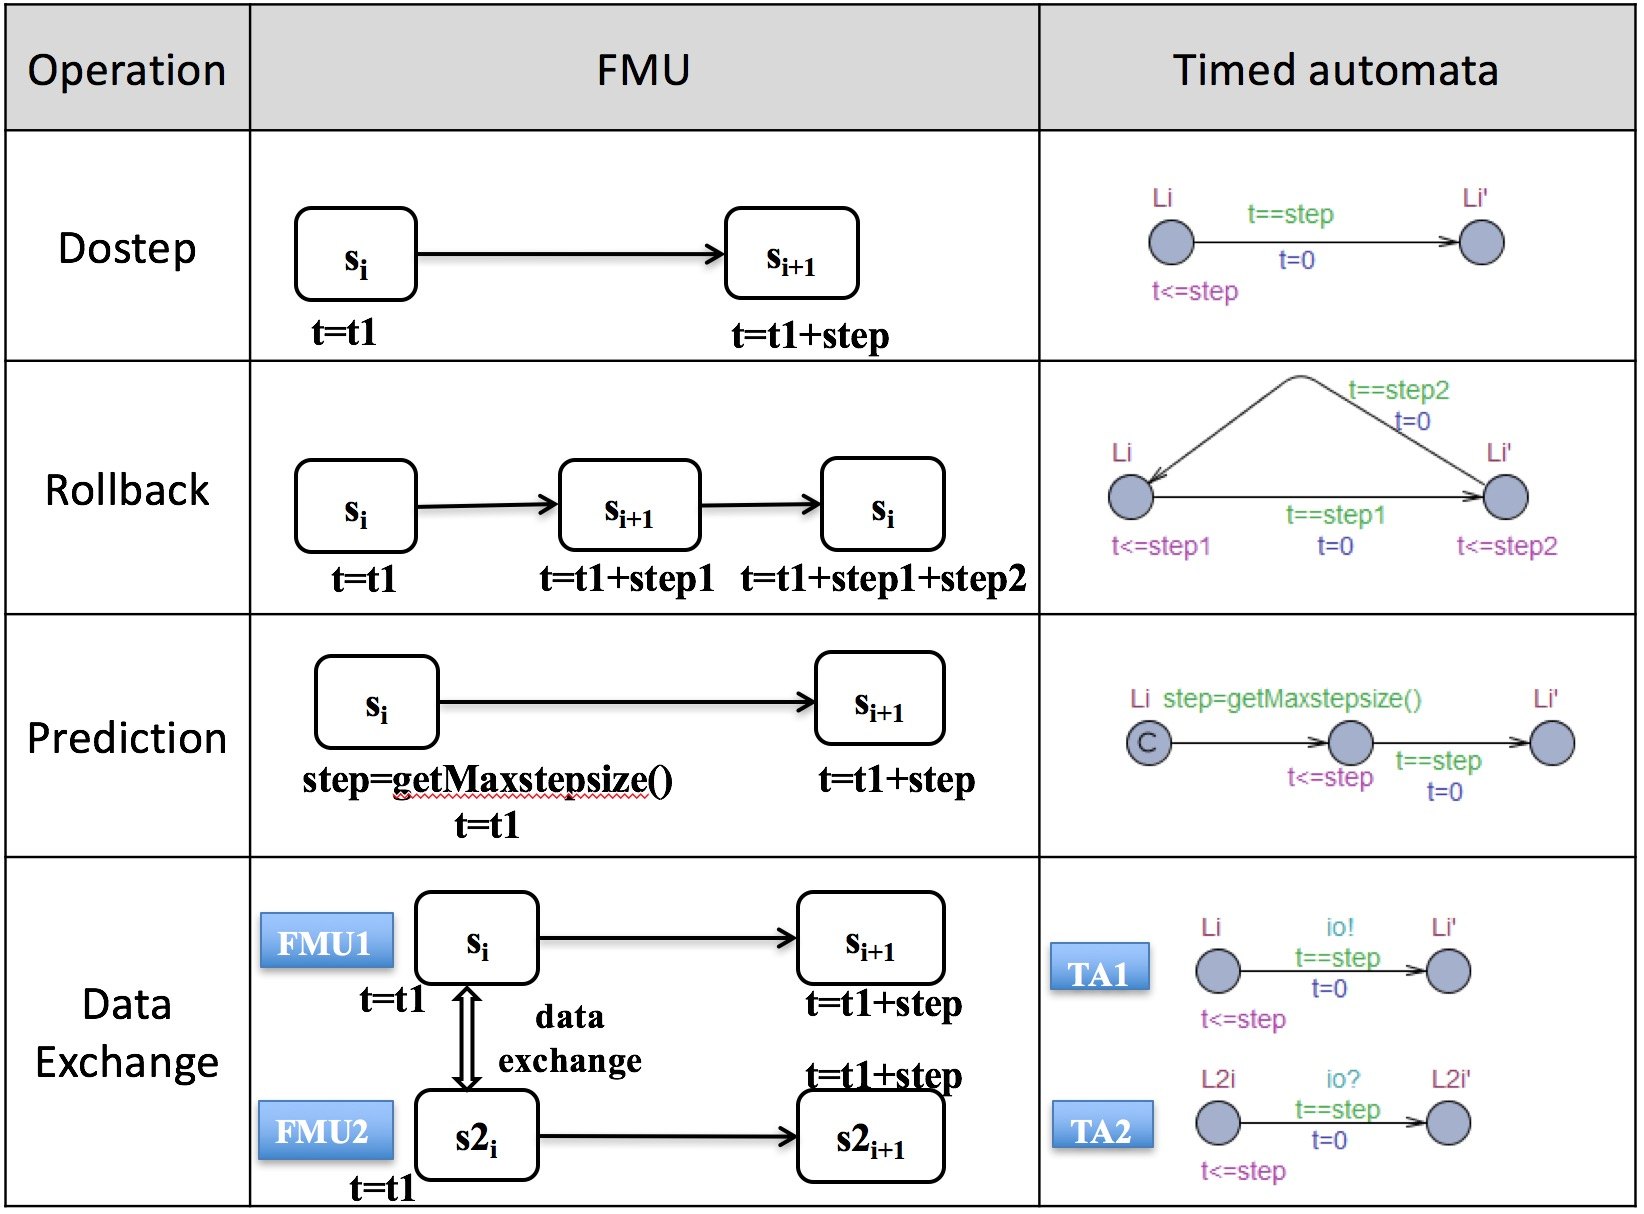
\includegraphics[width=3.5in,height=2.5in]{fig/abstractRole.png}}
	\caption{Abstraction rules from FMU to TA.}
	\label{fmutota}
\end{figure}
%\begin{algorithm}
%\caption{Encoding FMUs by timed automata}
%\label{alg:stuff}
%\begin{algorithmic}[1]
%\REQUIRE {$FMU=(S,U,Y,D,s_{0},set,get,doStep)$}
%\ENSURE {$\textit{TA}=(L,X,l_{0},E,E_{O},E_{I},I)$}
%\STATE TA.S $\gets$ FMU.S
%
%\end{algorithmic}
%%\end{algorithm}
%\end{algorithm}
As we can see from the Fig.\ref{fmutota}, given the current location $L_{i}$ at $t_{1}$, the operation $Dostep$ makes FMU reach a new location $L_{i+1}$ at $t_{1}+step$. The FMU can be transferred to a timed automata. A state $S_{i}$ goes to a new state $S_{i}^{\prime}$ after the step. In the operation $Rollback$, given the current location $L{i}$, the FMU will do a step to $L_{i+1}$, and then, the operation $rollback$ makes FMU reach the former location $L_{i}$. In TA, a state $S_{i}$ goes to a new state $S_{i}^{\prime}$ after a step, next returns to the former state $S_{i}$. In the operation prediction, when at the current location $L_{i}$, FMU can get Max step size, and reach a new location $L_{i+1}$. In TA, the state $S_{i}$ goes to a new state $S_{i}^{\prime}$ by the max step size. There is a data exchange between two FMUs at $t_{1}$, then they do the same step to $L_{i+1}$. In TA, there will be a signal to make the two FMUs do the same step from $S_{i}$ to $S_{i+1}$.
Although there are semantic gaps between FMUs and timed automata, we provide an appropriate transformation above to solve the problem. So, we believe that it's feasible to encode the FMUs by timed automata. In the following sections, we will model the FMUs with the timed automata in UPPAAL.


